\documentclass {beamer}
\usepackage[utf8]{inputenc}
\usepackage{amsmath}
\usepackage{natbib}
\linespread{1}
\usepackage{mcode}
\usepackage[lighttt]{lmodern}
\usepackage{graphicx} 
\usepackage{epstopdf}
\usepackage{subfigure}
\usetheme{Warsaw}
\usepackage{array,multirow,makecell}
\newcolumntype{M}[1]{>{\raggedright}m{#1}}
\title{\LARGE{Polymer Chain Dynamics Simulation}}
\author{Chenyu ZHA}

\begin{document}
\maketitle
\pagebreak
\AtBeginSection[]
{
  \begin{frame}
  \frametitle{Sommaire}
  \tableofcontents[currentsection]
  \end{frame} 
}
\section{The mean enounter time simulation}
	\begin{frame}
	\begin{columns}
		\begin{column}{0.5\textwidth}
		\begin{figure}
		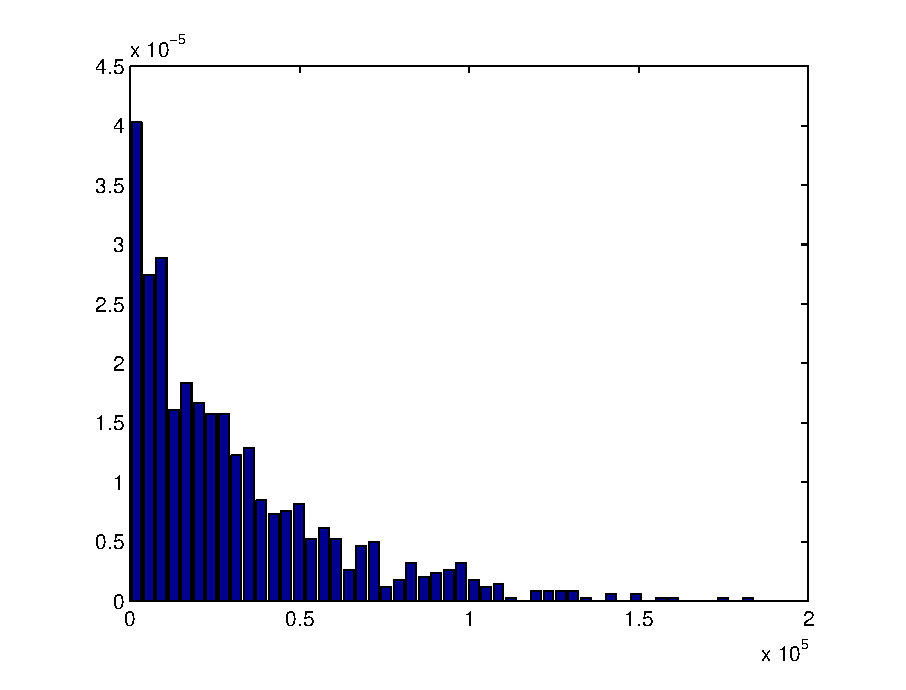
\includegraphics[width=1.3\textwidth]{MetTime4.eps}
		\end{figure}		
		\end{column}
		\begin{column}{0.3\textwidth}
		dimension = 3;
		numParticles = 1000;
		dt = 0.01;
		diffusionConst = 1;
		numSteps = Inf;
		\alert{numSimulations = 1000};
		frictionCoefficient = 1;
		connectedBeads = [];
		fixedBeads = [];
		metBeedNum = [1 16 32];
		lengthBead = 1;
		\alert{encounterDistance = b./5};
	   
		\end{column}
		\end{columns}
     	\end{frame}
	\begin{frame}
	\begin{columns}
		\begin{column}{0.5\textwidth}
		\begin{figure}
		%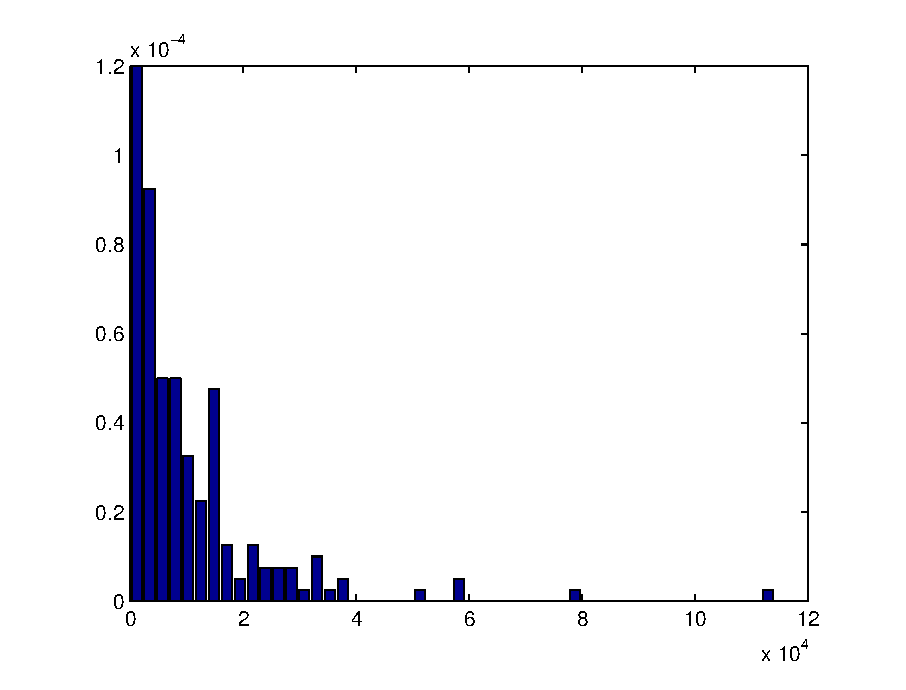
\includegraphics[width=1.3\textwidth]{MetTime5.eps}
		\end{figure}		
		\end{column}
		\begin{column}{0.3\textwidth}
		dimension = 3;
		numParticles = 1000;
		dt = 0.01;
		diffusionConst = 1;
		numSteps = Inf;
		\alert{numSimulations = 200};
		frictionCoefficient = 1;
		connectedBeads = [];
		fixedBeads = [];
		metBeedNum = [1 16 32];
		lengthBead = 1;
		\alert {encounterDistance = b./4};
	   
		\end{column}
		\end{columns}
     	\end{frame}
\section{End to End vector Simulation in the Rouse Model}
\begin{frame}
	\begin{columns}
		\begin{column}{0.5\textwidth}
		\begin{figure}
		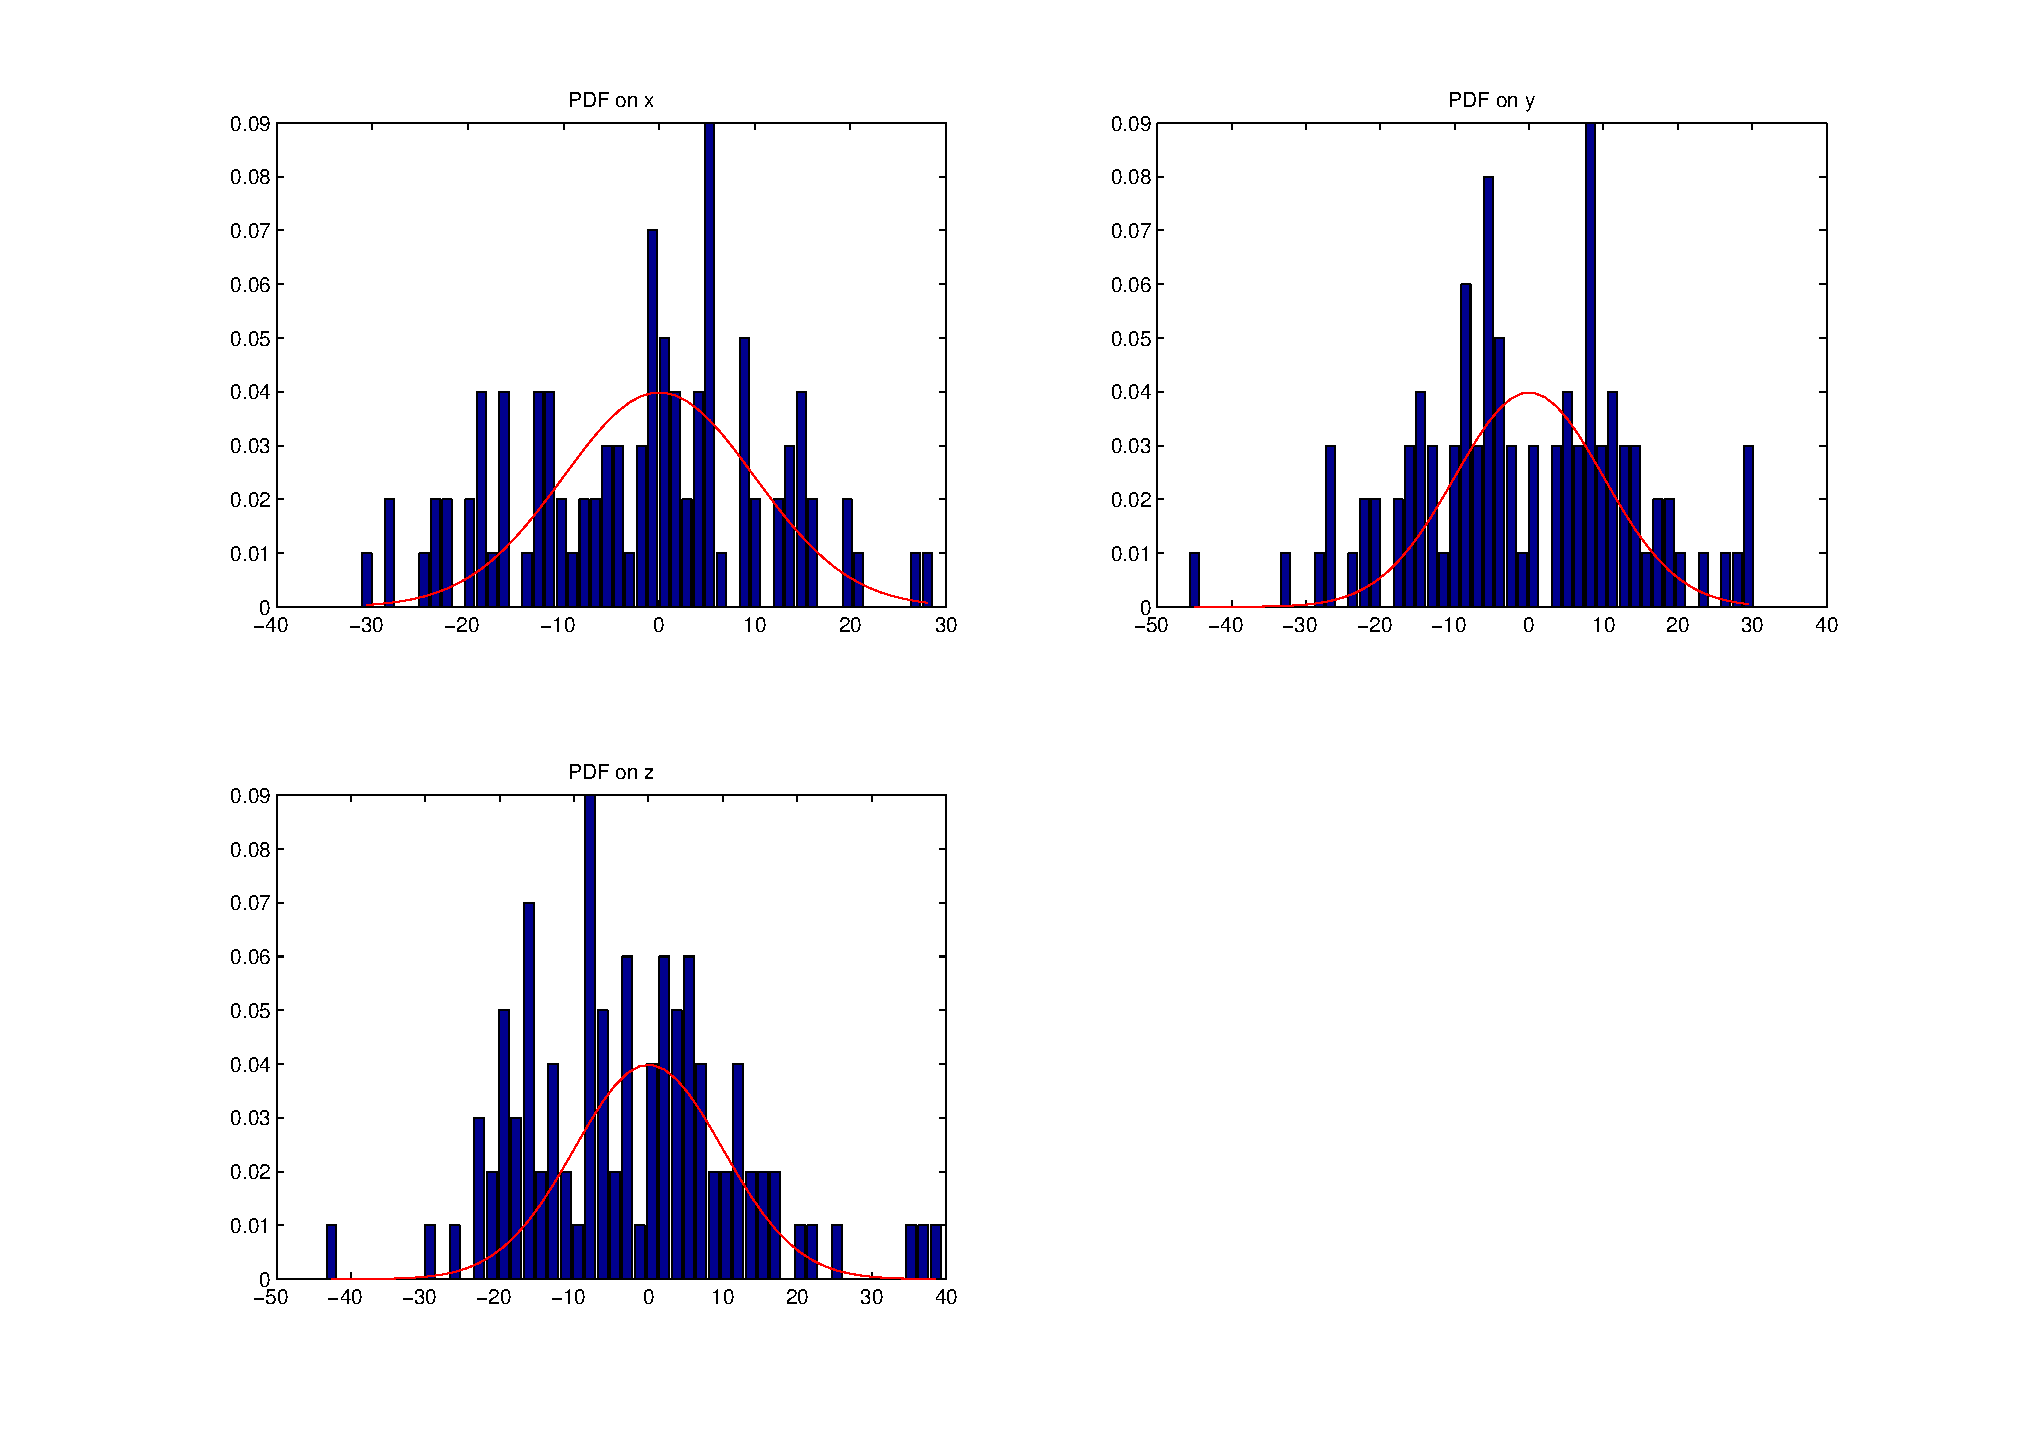
\includegraphics[width=1.3\textwidth]{PDF.eps}
		\end{figure}		
		\end{column}
		\begin{column}{0.3\textwidth}
		dimension=3
		numParticles=100
		dt=0.1
		numSteps=100
		diffusionConst=1
		paths %the paths of polymer;
		endToEndDist %end to end distance 
		simulation=100
		\end{column}
		\end{columns}
     	\end{frame}
\section{Random walk simulation}
\begin{frame}
\begin{columns}
		\begin{column}{0.5\textwidth}
		\begin{figure}
		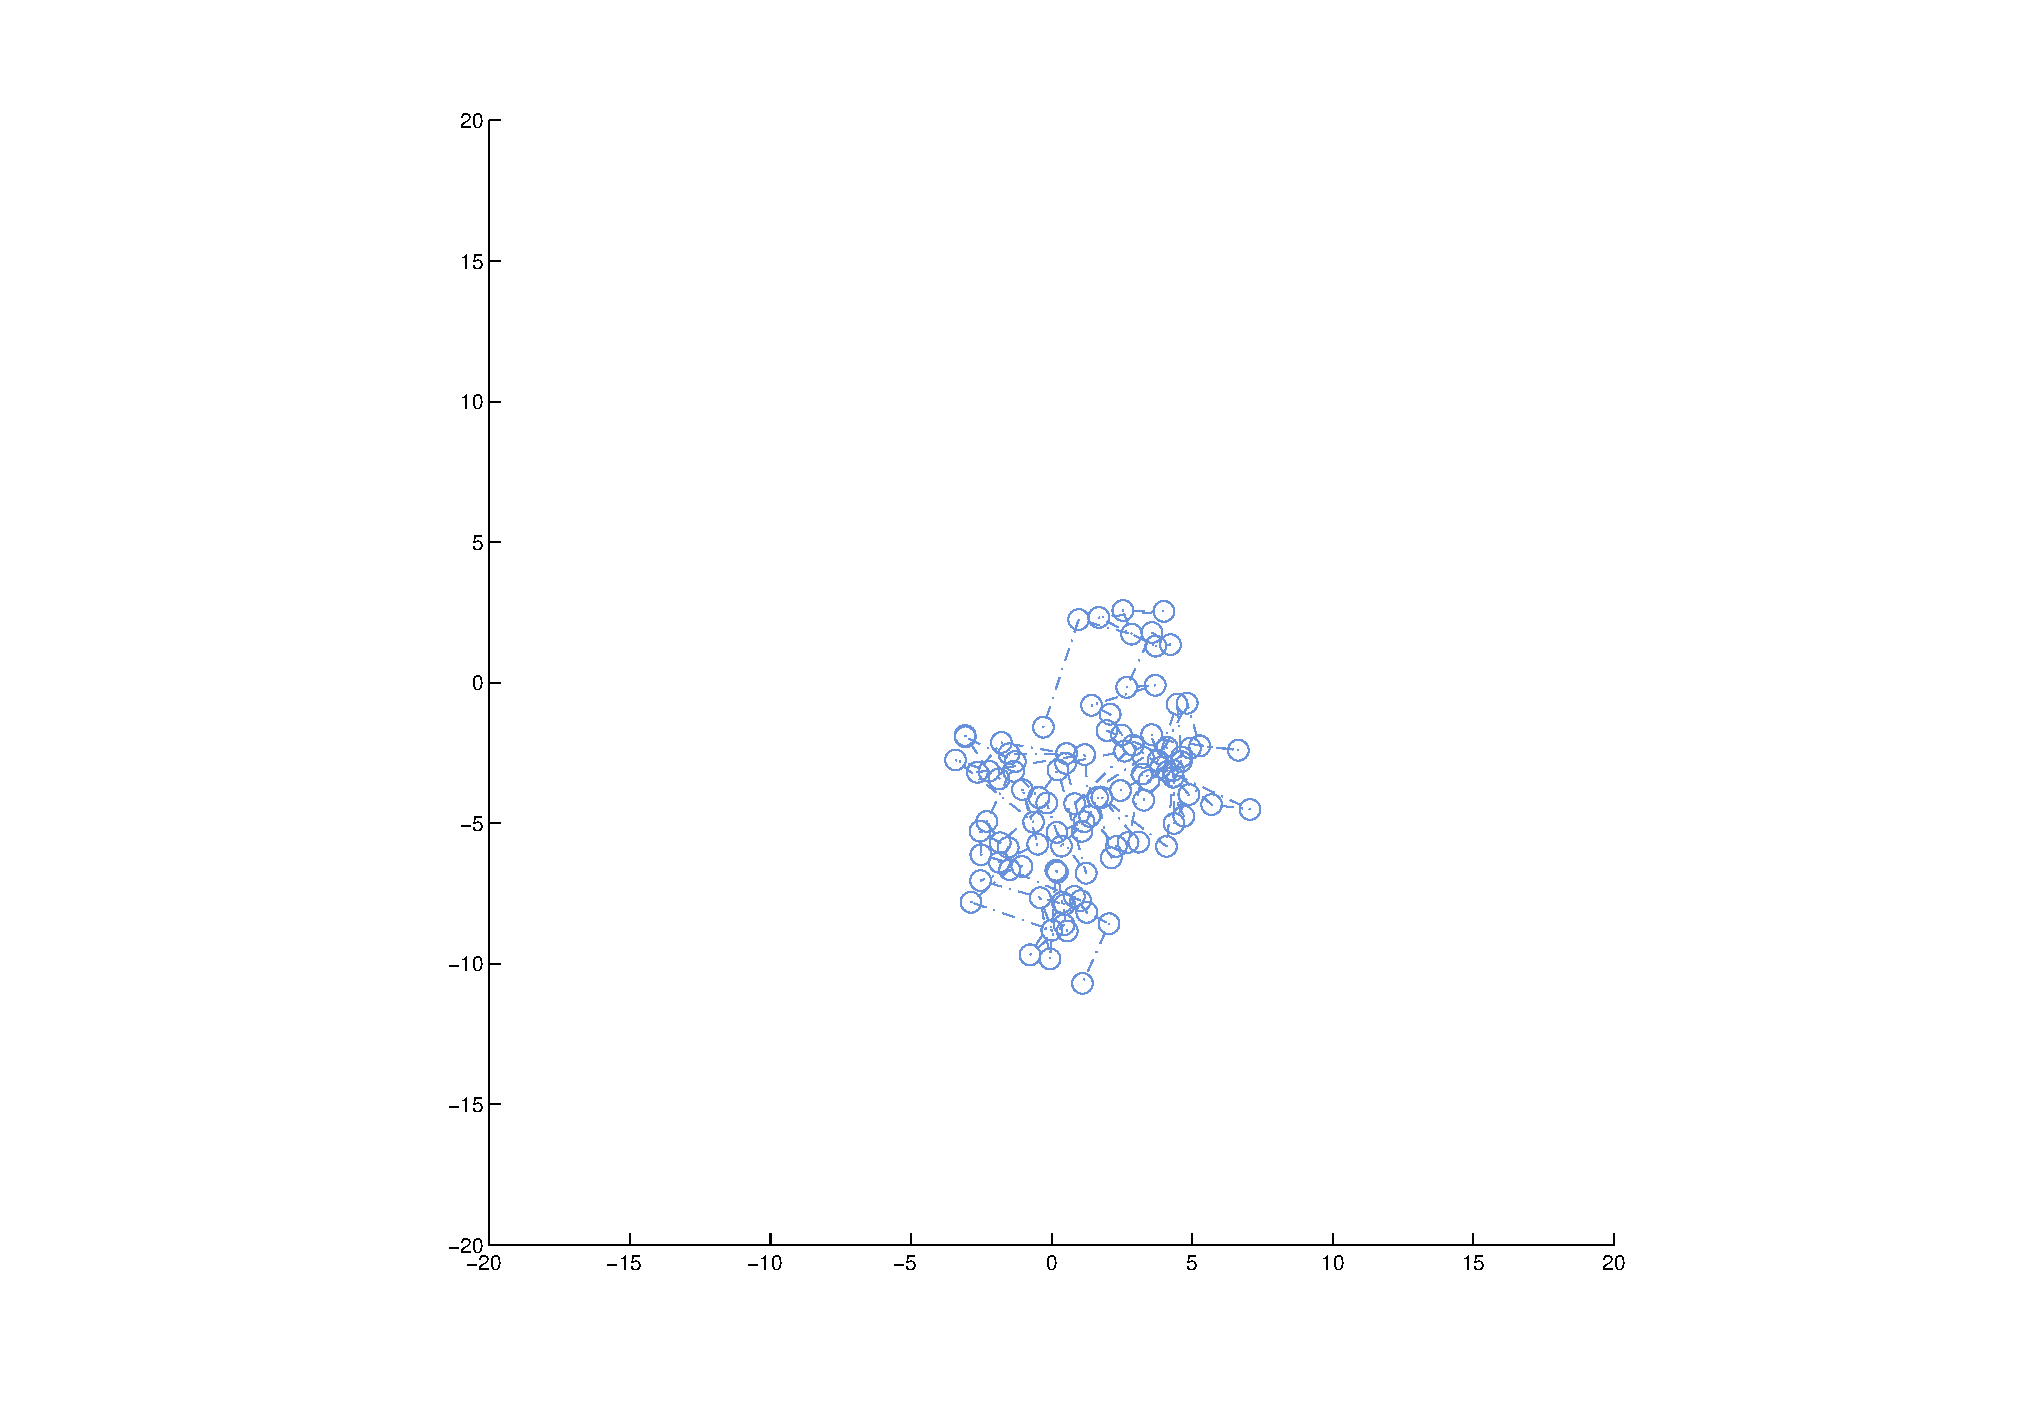
\includegraphics[width=1.0\textwidth]{1.eps}
		\caption{initial position}
		\end{figure}		
		\end{column}
		\begin{column}{0.3\textwidth}
			\begin{figure}
		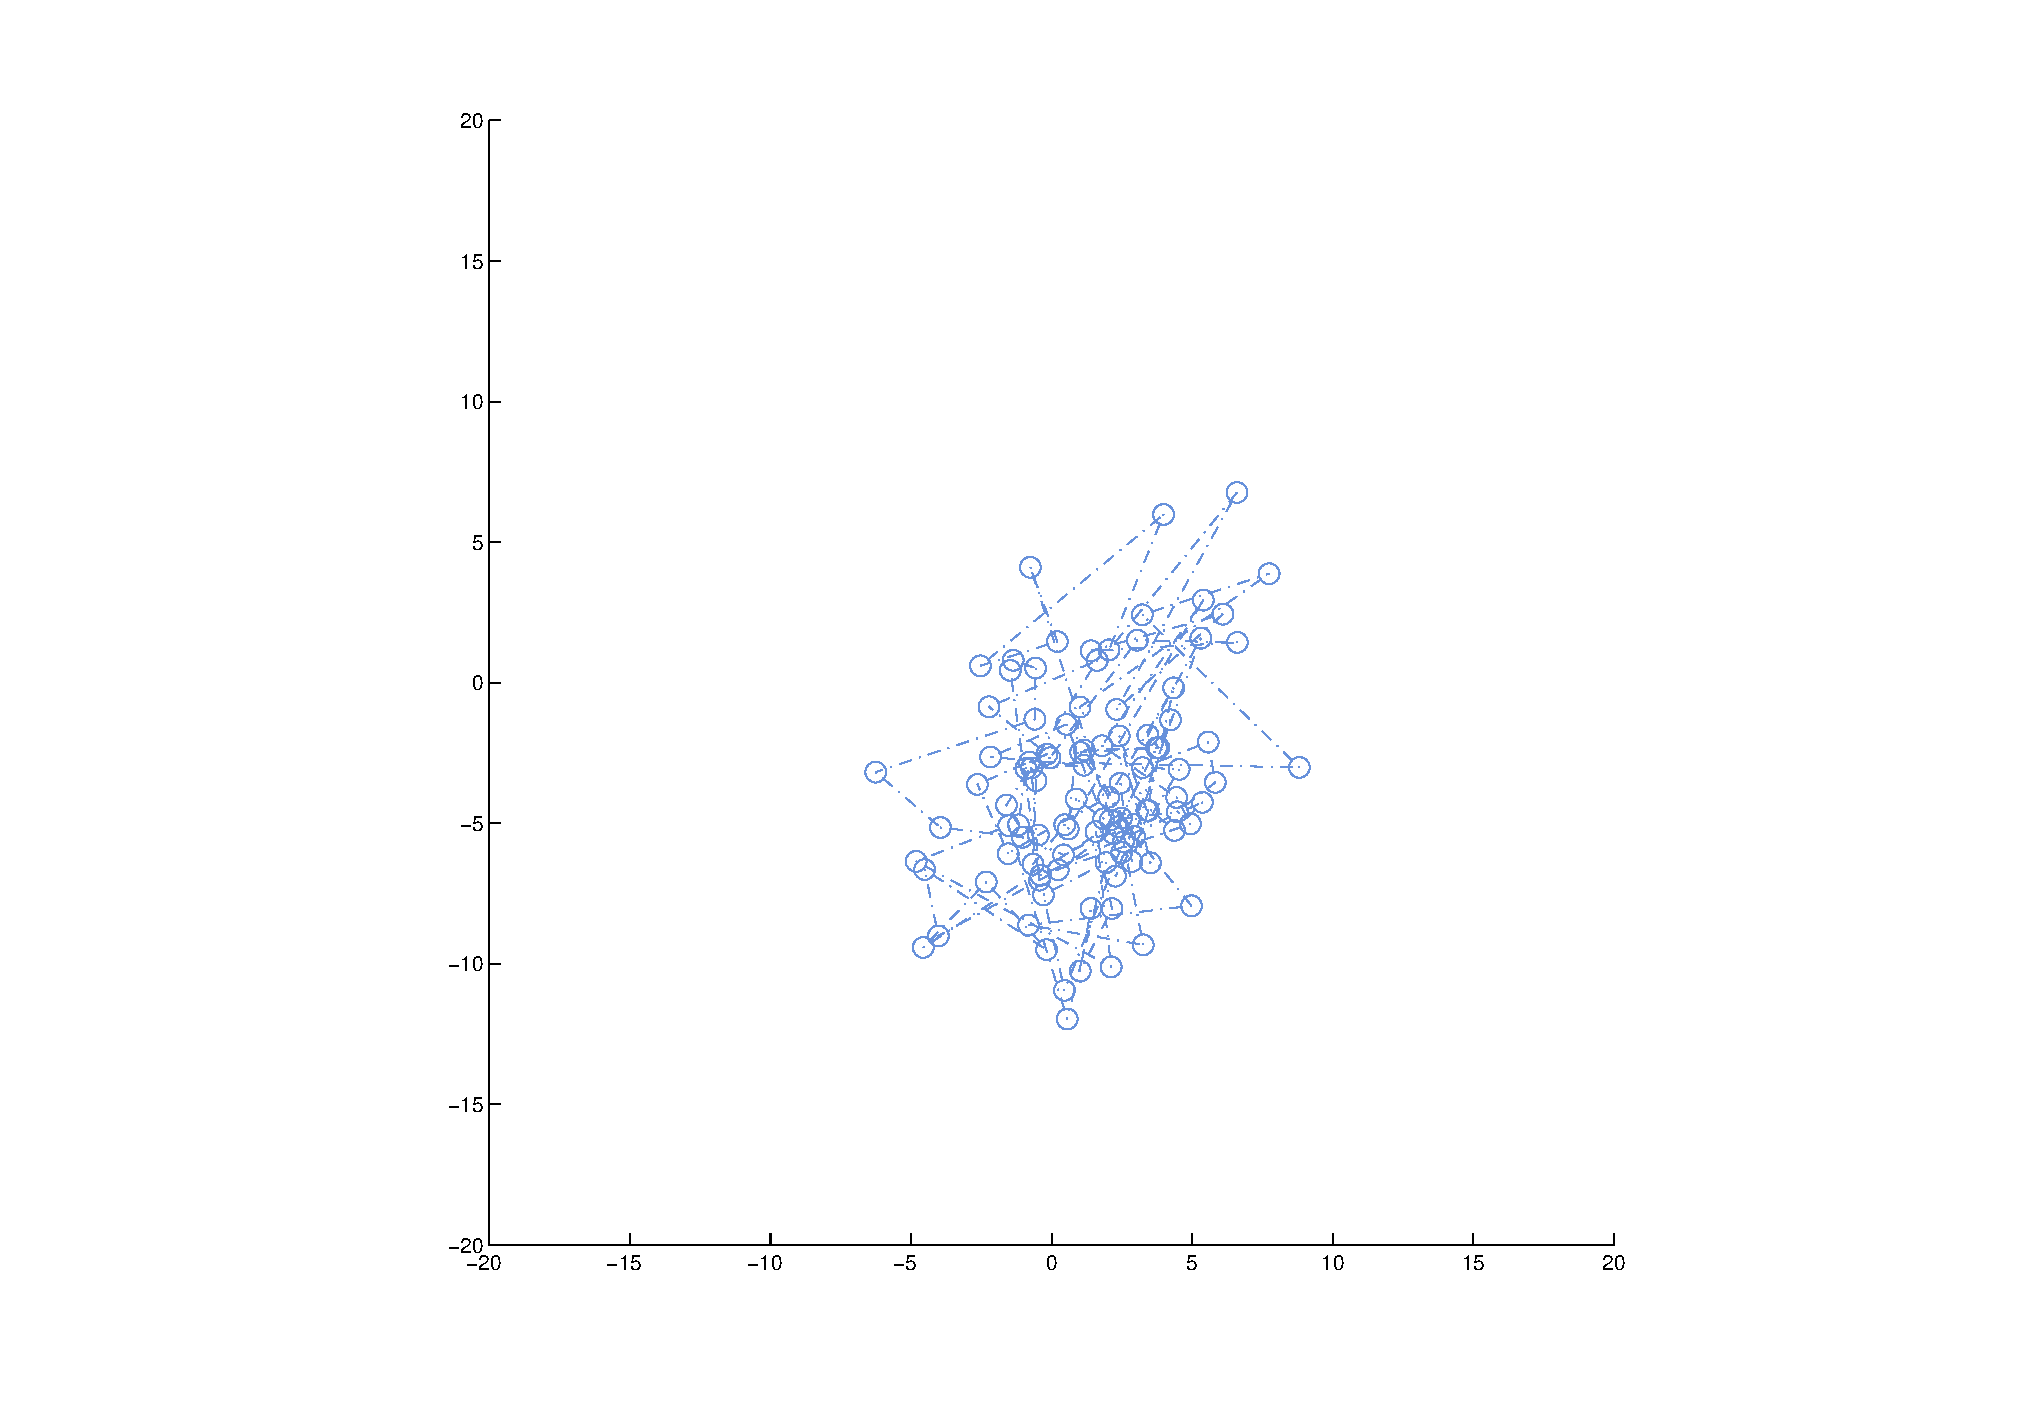
\includegraphics[width=1.5\textwidth]{2.eps}
		\caption{final position}
		\end{figure}		
		\end{column}
		\end{columns}
		parameters:dimension=3;numParticles=50;dt=0.1;\\numSteps=50;diffusionConst=1
		\end{frame}
\section{Perspective}		 
		 \begin{frame}
		 \begin{itemize}
		 \item Simulation on general domains
		 \item Simulate telometre clustering(sphere)
		 \item Build 'Results' module
		 \end{itemize}
		 \end{frame}
\end{document}